 \documentclass[c]{beamer}
%\documentclass{beamer}
\listfiles

\mode<presentation>
{
  %\usetheme[deutsch,titlepage0]{KIT}
\usetheme[deutsch]{KIT}
% \usetheme{KIT}

%%  \usefonttheme{structurebold}

  \setbeamercovered{transparent}

  \setbeamertemplate{enumerate items}[circle]
  %\setbeamertemplate{enumerate items}[ball]

}
\usepackage{babel}
\date{}
%\DateText

\newlength{\Ku}
\setlength{\Ku}{1.43375pt}

\usepackage[utf8]{inputenc}
\usepackage[TS1,T1]{fontenc}
\usepackage{array}
\usepackage{multicol}
\usepackage{lipsum}
\usepackage[]{algorithm2e}
\usepackage{amsmath}
\usepackage{color}

\usenavigationsymbols
%\usenavigationsymbols[sfHhdb]
%\usenavigationsymbols[sfhHb]

\subtitle{Algorithmen I SS 14}
\author[]{Lena Winter}

\AuthorTitleSep{\relax}

\institute[ITI]{Institut für Theoretische Informatik}

\TitleImage[width=\titleimagewd]{images/title}

\newlength{\tmplen}

\newcommand{\verysmall}{\fontsize{6pt}{8.6pt}\selectfont}

\title[Algorithmen I SS 14]{Tutorium 5}

\usepackage{alltt}

\TitleImage[width=\titleimagewd]{images/title}

\definecolor{english}{rgb}{0.0, 0.5, 0.0}

\begin{document}

\begin{frame}
  \maketitle
\end{frame}

\begin{frame}
	\begin{center}
		\Huge
		Sortieren (immer noch)
	\end{center}
\end{frame}

\begin{frame}{Bucket Sort}
	\begin{itemize}
		\item Array aus anfänglich leeren Buckets, denen jeweils ein Schlüssel zugewiesen ist
		\item Basierend auf den Schlüsseln werden die Elemente in die Buckets sortiert
	\end{itemize}

	\begin{block}{Eigenschaften}
		\begin{itemize}
			\item {\color{english}{stabil}}
			\item {\color{red}{nicht inplace}}
			\item Laufzeit $\mathcal{O}(n+k)$
		\end{itemize}
	\end{block}


	$\Rightarrow$ Sinnvoll bei kleiner Schlüsselmenge

\end{frame}

\begin{frame}{Radix Sort}

	Nutze Stabilität von Bucket Sort: Sortieren nacheinander nach einzelnen Ziffern

	\begin{block}{Mehrere Varianten}
	\begin{itemize}
		\item Beginnend beim Most Significant Digit (MSD)
		\item Beginnend beim Least Significant Digit (LSD)
	\end{itemize}
	\end{block}

	\begin{block}{Eigenschaften}
		\begin{itemize}
			\item {\color{english}{stabil}}
			\item {\color{red}{nicht inplace}}
			\item Laufzeit $\mathcal{O}(d * (n + k))$ für $d =$ Anzahl digits
		\end{itemize}
	\end{block}

	\begin{block}{Beispiel}
		$\langle 978, 557, 963, 587, 718, 863, 497 \rangle $
	\end{block}
\end{frame}

\begin{frame}{Vergleichsbasiert vs. Nicht Vergleichsbasiert}

	{\textbf{\large{Pro Nicht Vergleichsbasiert:}}}
	\begin{itemize}
		\item asymptotisch schneller
	\end{itemize}


	{\textbf{\large{Pro Vergleichsbasiert:}}} \\
	\begin{itemize}
		\item weniger Voraussetzungen an die zu sortierenden Elemente
		\item Cache-Effizienz weniger schwierig
		\item bei langen Schlüsseln oft schneller
		\item robust gegen beliebige Eingabeverteilungen
	\end{itemize}

\end{frame}
\begin{frame}
	\begin{center}
		\Huge
		Partitionierung bei Quicksort
	\end{center}
\end{frame}

\begin{frame}{Partitionierung mit Zeigern von beiden Seiten}
	\begin{itemize}
		\item Liste wird durch zwei Zeiger (i, j mit $ i \leq j $) in drei Teile unterteilt:
		\begin{itemize}
			\item am Anfang i = Anfang der Folge, j = Ende der Folge
			\item bis $i$: Elemente $< p$
			\item bis $j - 1$: unbetrachtete Elemente
			\item bis $r$: Elemente $\geq p$
		\end{itemize}
		\item Zeiger laufen aufeinander zu, solange die Zuteilung stimmt
		\item Sobald beide Zeiger bei falsch positionierten Elementen angekommen sind wird vertauscht
		\item Abbruch bei $i > j$
	\end{itemize}
\end{frame}

\begin{frame}{Partitionierung mit beiden Zeigern von links}
	\begin{itemize}
		\item Pivotelement (p) steht an der letzten Stelle der Folge (r)
		\item Folge wird durch zwei Zeiger (i, j mit $ i \leq j $) in drei Teile unterteilt:
		\begin{itemize}
			\item am Anfang i = j = Anfang der Folge
			\item bis $i - 1$: Elemente $\leq$ p
			\item bis $j - 1$: Elemente > p
			\item bis $r - 1$: unbetrachtete Elemente
		\end{itemize}
		\item Wenn Element an der $j$-ten Stelle $\leq p$, dann tausche die Elemente an Stelle $i$ und $j$ und inkrementiere $i$
		\item inkrementiere j
		\item Wenn j bei $r-1$ ankommt, vertausche Element bei $r$ mit Element bei $i$
	\end{itemize}
\end{frame}

\begin{frame} {Quicksort: Worst Case}
	Worst case bei Quicksort $\Leftrightarrow$ Pivot ist immer Max/Min

	\begin{exampleblock}{Gedankenspiel:}
		Array bestehenend aus nur gleichen Elementen: $\langle 2, 2, 2, 2 \rangle $
	\end{exampleblock}

	$\Rightarrow$ Standard-Quicksort schlecht bei vielen gleichen Elementen
\end{frame}

\begin{frame}{Stattdessen: 3-way-partition}
	\begin{itemize}
		\item 3 Pointer: i, j ,k
			\begin{itemize}
				\item bis i - 1: Elemente $< p$
				\item bis j - 1: Elemente $> p$
				\item bis k: unbetrachtete Elemente
				\item bis r: Elemente $= p$
			\end{itemize}
		\item Wie 2-way von links
		\item Außer: Wenn Element an $j$-ter Stelle $= p$, tausche mit $k$-tem Element und inkrementiere $j$ \emph{nicht}
		\item Am Ende den ($ = p$) Teil zwischen ($< p$) und ($> p$) schieben.
	\end{itemize}

\end{frame}


\begin{frame}{Beispiel Partition}
	Partitioniere \(\langle 16, 52, 50, 17, 80, 27, 29, 21, 23, 29, 17, 33, 50, 83 \rangle\) (29 als Pivot) mit

	\begin{enumerate}
		\item von beiden Seiten
		\item von links
		\item 3-way von links
	\end{enumerate}
\end{frame}

\begin{frame}
	\begin{center}
		\Huge
		Quickselect
	\end{center}
\end{frame}

\begin{frame}{Quickselect}
	\begin{itemize}
		\item \textbf{Rang} eines Elements: Position des Elements in der sortierten Folge
		\item Nicht eindeutig bei mehreren gleichen Elementen!
		\item Gesucht: \emph{select(s, k)} soll das Element mit Rang \emph{k} in der (unsortierten) Folge \emph{s} liefern
		\item Lösung: (einseitiges) Quicksort
		\item Erwartet \(\mathcal{O}(n)\), Worst-Case \(\mathcal{O}(n^2)\)
	\end{itemize}
\end{frame}

\begin{frame}{Quickselect}
	Ziel: Element mit Rang \emph{k}
	\begin{enumerate}
		\item Wähle ein Pivot-Element
		\item Partitioniere Folge wie bei Quicksort in \emph{a} (<), \emph{b} (=), \emph{c} (>)
		\item Vergleiche Größe von Teillisten mit Rang:
			\begin{itemize}
				\item Element in \emph{a}: return \emph{select(a, k)}
				\item Element in \emph{b}: return Pivot
				\item Element in \emph{c}: return \emph{select(c, $k - |a| - |b|$)}
			\end{itemize}
	\end{enumerate}
\end{frame}

\begin{frame}{Beispiel Quickselect}
	\(s = \langle 45, 31, 93, 30, 5, 67, 0, 39, 19, 41, 45 \rangle\)

	Finde das Element mit Rang 7 mit Quickselect (erstes Element als Pivot)
\end{frame}

\begin{frame}
	\frametitle{Seat Selection}
	\begin{center}
		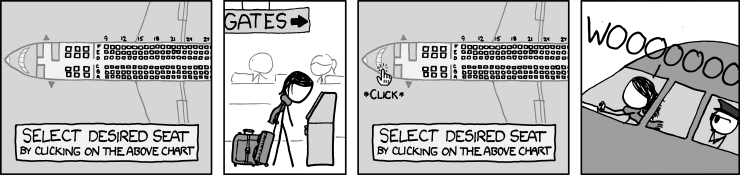
\includegraphics[width=\textwidth,height=\textheight,keepaspectratio]{images/seat_selection}
	\end{center}
\end{frame}

\end{document}
